% questions.tex —— 2015 年·全国Ⅱ卷·文科 · 题目内容片段（无答案）
% 由 tools/generate_projects.py 依来源总账自 2015/2015_数学真题_全国2文_试题.md 生成，勿手改（改源 MD 后重跑）


\begin{gktip}
据固定原卷照录，不添加原卷未印出的分值、满分和时长。题图是源图矢量描绘，示意坐标不作原始数据。
\end{gktip}

\gkpart{一、选择题}

\begin{question}
\gkti{1}已知集合 $A=\{x\mid -1<x<2\}$，$B=\{x\mid 0<x<3\}$，则 $A\cup B=$（　）

(A) $(-1,3)$　(B) $(-1,0)$　(C) $(0,2)$　(D) $(2,3)$

\end{question}
\begin{question}
\gkti{2}若 $a$ 为实数，且 $\dfrac{2+ai}{1+i}=3+i$，则 $a=$（　）

(A) $-4$　(B) $-3$　(C) $3$　(D) $4$

\Needspace{0.4\textheight}
\end{question}
\begin{question}
\gkti{3}根据下面给出的 2004 年至 2013 年我国二氧化硫年排放量（单位：万吨）柱形图，以下结论中不正确的是（　）
\nopagebreak[4]
\begin{center}% FIG:q03-emissions
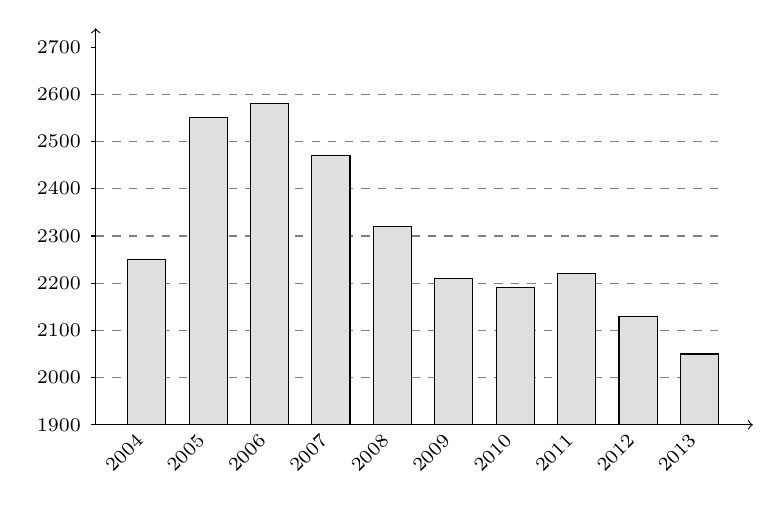
\begin{tikzpicture}[x=0.78cm,y=0.006cm,line width=0.4pt]
  % Approximate bar heights transcribed from the source image, not exact data.
  \draw[->] (0,1900) -- (10.7,1900);
  \draw[->] (0,1900) -- (0,2740);
  \foreach \y in {1900,2000,...,2700} {
    \draw (0,\y) -- (-0.08,\y) node[left] {\scriptsize \y};
  }
  \foreach \y in {2000,2100,...,2600} {
    \draw[dashed,gray] (0,\y) -- (10.2,\y);
  }
  \draw (0,1900) -- (10.2,1900);
  \foreach \i/\year/\v in {
    0/2004/2250,1/2005/2550,2/2006/2580,3/2007/2470,4/2008/2320,
    5/2009/2210,6/2010/2190,7/2011/2220,8/2012/2130,9/2013/2050} {
    \pgfmathsetmacro{\x}{0.52+\i}
    \draw[fill=gray!25] (\x,1900) rectangle ++(0.62,\v-1900);
    \node[below=2pt,rotate=45,anchor=east] at (\x+0.31,1900) {\scriptsize \year};
  }
\end{tikzpicture}
\end{center}
\nopagebreak[4]
(A) 逐年比较，2008 年减少二氧化硫排放量的效果最显著  
(B) 2007 年我国治理二氧化硫排放显现成效  
(C) 2006 年以来我国二氧化硫年排放量呈减少趋势  
(D) 2006 年以来我国二氧化硫年排放量与年份正相关

\end{question}
\begin{question}
\gkti{4}已知 $\boldsymbol a=(1,-1)$，$\boldsymbol b=(-1,2)$，则 $(2\boldsymbol a+\boldsymbol b)\cdot\boldsymbol a=$（　）

(A) $-1$　(B) $0$　(C) $1$　(D) $2$

\end{question}
\begin{question}
\gkti{5}设 $S_n$ 是等差数列 $\{a_n\}$ 的前 $n$ 项和，若 $a_1+a_3+a_5=3$，则 $S_5=$（　）

(A) $5$　(B) $7$　(C) $9$　(D) $11$

\Needspace{0.4\textheight}
\end{question}
\begin{question}
\gkti{6}一个正方体被一个平面截去一部分后，剩余部分的三视图如图，则截去部分体积与剩余部分体积的比值为（　）
\nopagebreak[4]
\begin{center}% FIG:q06-three-views
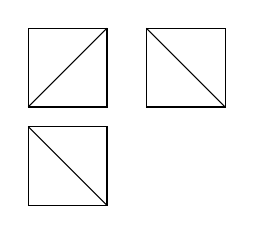
\begin{tikzpicture}[x=1cm,y=1cm,line width=0.4pt]
  \draw (0,1.25) rectangle (1,2.25);
  \draw (0,1.25) -- (1,2.25);
  \draw (1.5,1.25) rectangle (2.5,2.25);
  \draw (1.5,2.25) -- (2.5,1.25);
  \draw (0,0) rectangle (1,1);
  \draw (0,1) -- (1,0);
\end{tikzpicture}
\end{center}
\nopagebreak[4]
(A) $\dfrac18$　(B) $\dfrac17$　(C) $\dfrac16$　(D) $\dfrac15$

\end{question}
\begin{question}
\gkti{7}已知三点 $A(1,0)$，$B(0,\sqrt3)$，$C(2,\sqrt3)$，则 $\triangle ABC$ 外接圆的圆心到原点的距离为（　）

(A) $\dfrac53$　(B) $\dfrac{\sqrt{21}}3$　(C) $\dfrac{2\sqrt5}3$　(D) $\dfrac43$

\Needspace{0.4\textheight}
\end{question}
\begin{question}
\gkti{8}下边程序框图的算法思路源于我国古代数学名著《九章算术》中的“更相减损术”。执行该程序框图，若输入的 $a,b$ 分别为 $14,18$，则输出的 $a=$（　）
\nopagebreak[4]
\begin{center}% FIG:q08-flowchart
\begin{tikzpicture}[>=stealth,line width=0.45pt,
  every node/.style={font=\small,align=center},
  terminal/.style={draw,rounded corners,minimum width=1.05cm,minimum height=0.48cm},
  io/.style={draw,minimum width=1.55cm,minimum height=0.5cm,shape=trapezium,trapezium left angle=70,trapezium right angle=110},
  decision/.style={draw,diamond,aspect=2.1,inner sep=1pt,minimum width=1.45cm,minimum height=0.7cm},
  process/.style={draw,minimum width=1.45cm,minimum height=0.48cm}]
  \node[terminal] (start) at (0,4.5) {开始};
  \node[io] (input) at (0,3.65) {输入 $a,b$};
  \node[decision] (neq) at (0,2.65) {$a\ne b$};
  \node[decision] (gt) at (0,1.25) {$a>b$};
  \node[io] (out) at (2.25,2.65) {输出 $a$};
  \node[terminal] (end) at (2.25,1.75) {结束};
  \node[process] (suba) at (-1.55,0.05) {$a=a-b$};
  \node[process] (subb) at (1.55,0.05) {$b=b-a$};
  \draw[->] (start) -- (input);
  \draw[->] (input) -- (neq);
  \draw[->] (neq.east) -- node[above]{否} (out.west);
  \draw[->] (out) -- (end);
  \draw[->] (neq.south) -- node[right]{是} (gt.north);
  \draw[->] (gt.south west) -- node[above left]{是} (suba.north);
  \draw[->] (gt.south east) -- node[above right]{否} (subb.north);
  \draw[->] (suba.south) -- (-1.55,-0.65);
  \draw[->] (subb.south) -- (1.55,-0.65);
  \draw (-1.55,-0.65) -- (1.55,-0.65);
  \draw[->] (-1.55,-0.65) -- (-3.6,-0.65) -- (-3.6,2.65) -- (neq.west);
\end{tikzpicture}
\end{center}
\nopagebreak[4]
(A) $0$　(B) $2$　(C) $4$　(D) $14$

\end{question}
\begin{question}
\gkti{9}已知等比数列 $\{a_n\}$ 满足 $a_1=\dfrac14$，$a_3a_5=4(a_4-1)$，则 $a_2=$（　）

(A) $2$　(B) $1$　(C) $\dfrac12$　(D) $\dfrac18$

\end{question}
\begin{question}
\gkti{10}已知 $A,B$ 是球 $O$ 的球面上两点，$\angle AOB=90^\circ$，$C$ 为该球面上的动点，若三棱锥 $O-ABC$ 体积的最大值为 $36$，则球 $O$ 的表面积为（　）

(A) $36\pi$　(B) $64\pi$　(C) $144\pi$　(D) $256\pi$

\Needspace{0.4\textheight}
\end{question}
\begin{question}
\gkti{11}如图，长方形 $ABCD$ 的边 $AB=2$，$BC=1$，$O$ 是 $AB$ 的中点，点 $P$ 沿着边 $BC,CD$ 与 $DA$ 运动，记 $\angle BOP=x$。将动点 $P$ 到 $A,B$ 两点距离之和表示为 $x$ 的函数 $f(x)$，则 $y=f(x)$ 的图象大致为（　）
\nopagebreak[4]
\begin{center}% FIG:q11-rectangle
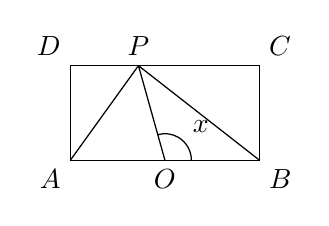
\begin{tikzpicture}[x=1.2cm,y=1.2cm,line width=0.45pt]
  \coordinate (A) at (0,0);
  \coordinate (B) at (2,0);
  \coordinate (C) at (2,1);
  \coordinate (D) at (0,1);
  \coordinate (O) at (1,0);
  \coordinate (P) at (0.72,1);
  \draw (A) -- (B) -- (C) -- (D) -- cycle;
  \draw (P) -- (A) (P) -- (O) (P) -- (B);
  \draw (A) node[below left] {$A$} (B) node[below right] {$B$}
    (C) node[above right] {$C$} (D) node[above left] {$D$}
    (O) node[below] {$O$} (P) node[above] {$P$};
  \draw (O) ++(0:0.28) arc[start angle=0,end angle=106,radius=0.28];
  \node at (1.38,0.36) {$x$};
\end{tikzpicture}
\end{center}
\nopagebreak[4]
\nopagebreak[4]
\begin{center}% FIG:q11-option-a
\begin{tikzpicture}[x=0.9cm,y=0.85cm,line width=0.45pt]
  \draw[->] (0,0) -- (4.45,0) node[right] {$x$};
  \draw[->] (0,0) -- (0,2.65) node[above] {$y$};
  \foreach \x/\lab in {1/{\frac{\pi}{4}},2/{\frac{\pi}{2}},3/{\frac{3\pi}{4}},4/{\pi}} {
    \draw (\x,0) -- +(0,-0.06) node[below=2pt] {$\lab$};
  }
  \draw (-0.07,2) -- (0.07,2) node[left=4pt] {$2$};
  \node[below left] at (0,0) {$O$};
  \draw (0,2) -- (1,2.48) -- (2,2.2) -- (3,2.48) -- (4,2);
\end{tikzpicture}
\end{center}
\nopagebreak[4]
\nopagebreak[4]
\begin{center}% FIG:q11-option-b
\begin{tikzpicture}[x=0.9cm,y=0.85cm,line width=0.45pt]
  \draw[->] (0,0) -- (4.45,0) node[right] {$x$};
  \draw[->] (0,0) -- (0,2.65) node[above] {$y$};
  \foreach \x/\lab in {1/{\frac{\pi}{4}},2/{\frac{\pi}{2}},3/{\frac{3\pi}{4}},4/{\pi}} {
    \draw (\x,0) -- +(0,-0.06) node[below=2pt] {$\lab$};
  }
  \draw (-0.07,2) -- (0.07,2) node[left=4pt] {$2$};
  \node[below left] at (0,0) {$O$};
  \draw (0,2) .. controls (0.35,2.35) and (0.78,2.60) .. (1,2.55)
    .. controls (1.08,2.25) and (1.65,2.05) .. (2,2.1)
    .. controls (2.35,2.05) and (2.88,2.20) .. (3,2.55)
    .. controls (3.2,2.60) and (3.65,2.35) .. (4,2);
\end{tikzpicture}
\end{center}
\nopagebreak[4]
\nopagebreak[4]
\begin{center}% FIG:q11-option-c
\begin{tikzpicture}[x=0.9cm,y=0.85cm,line width=0.45pt]
  \draw[->] (0,0) -- (4.45,0) node[right] {$x$};
  \draw[->] (0,0) -- (0,2.65) node[above] {$y$};
  \foreach \x/\lab in {1/{\frac{\pi}{4}},2/{\frac{\pi}{2}},3/{\frac{3\pi}{4}},4/{\pi}} {
    \draw (\x,0) -- +(0,-0.06) node[below=2pt] {$\lab$};
  }
  \draw (-0.07,2) -- (0.07,2) node[left=4pt] {$2$};
  \node[below left] at (0,0) {$O$};
  \draw (0,2) -- (2,2.52) -- (4,2);
\end{tikzpicture}
\end{center}
\nopagebreak[4]
\nopagebreak[4]
\begin{center}% FIG:q11-option-d
\begin{tikzpicture}[x=0.9cm,y=0.85cm,line width=0.45pt]
  \draw[->] (0,0) -- (4.45,0) node[right] {$x$};
  \draw[->] (0,0) -- (0,2.65) node[above] {$y$};
  \foreach \x/\lab in {1/{\frac{\pi}{4}},2/{\frac{\pi}{2}},3/{\frac{3\pi}{4}},4/{\pi}} {
    \draw (\x,0) -- +(0,-0.06) node[below=2pt] {$\lab$};
  }
  \draw (-0.07,2) -- (0.07,2) node[left=4pt] {$2$};
  \node[below left] at (0,0) {$O$};
  \draw (0,2) arc[start angle=180,end angle=0,x radius=2cm,y radius=0.55cm];
\end{tikzpicture}
\end{center}
\nopagebreak[4]
\end{question}
\begin{question}
\gkti{12}设函数 $f(x)=\ln(1+|x|)-\dfrac1{1+x^2}$，则使得 $f(x)>f(2x-1)$ 成立的 $x$ 的取值范围是（　）

(A) $\left(\dfrac13,1\right)$　(B) $\left(-\infty,\dfrac13\right)\cup(1,+\infty)$  
(C) $\left(-\dfrac13,\dfrac13\right)$　(D) $\left(-\infty,-\dfrac13\right)\cup\left(\dfrac13,+\infty\right)$

\end{question}
\gkpart{二、填空题}

\begin{question}
\gkti{13}已知函数 $f(x)=ax^3-2x$ 的图象过点 $(-1,4)$，则 $a=$\gkblank{}。

\end{question}
\begin{question}
\gkti{14}若 $x,y$ 满足约束条件 $\begin{cases}x+y-5\le0,\\2x-y-1\ge0,\\x-2y+1\le0,\end{cases}$ 则 $z=2x+y$ 的最大值为\gkblank{}。

\end{question}
\begin{question}
\gkti{15}已知双曲线过点 $(4,\sqrt3)$，且渐近线方程为 $y=\pm\dfrac12x$，则该双曲线的标准方程为\gkblank{}。

\end{question}
\begin{question}
\gkti{16}已知曲线 $y=x+\ln x$ 在点 $(1,1)$ 处的切线与曲线 $y=ax^2+(a+2)x+1$ 相切，则 $a=$\gkblank{}。

\end{question}
\gkpart{三、解答题}

\begin{question}
\gkti{17}$\triangle ABC$ 中，$D$ 是 $BC$ 上的点，$AD$ 平分 $\angle BAC$，$BD=2DC$。

(1) 求 $\dfrac{\sin\angle B}{\sin\angle C}$；  
(2) 若 $\angle BAC=60^\circ$，求 $\angle B$。

\Needspace{0.4\textheight}
\end{question}
\begin{question}
\gkti{18}某公司为了了解用户对其产品的满意度，从 $A,B$ 两地区分别随机调查了 $40$ 个用户，根据用户对其产品的满意度的评分，得到 $A$ 地区用户满意度评分的频率分布直方图和 $B$ 地区用户满意度评分的频率分布表。

$A$ 地区用户满意度评分的频率分布直方图：
\nopagebreak[4]
\begin{center}% FIG:q18-a-histogram
\begin{tikzpicture}[x=0.105cm,y=115cm,line width=0.4pt]
  \draw[->] (36,0) -- (106,0) node[right] {满意度评分};
  \draw[->] (40,0) -- (40,0.044) node[above] {频率/组距};
  \foreach \x in {40,50,...,100} {
    \draw (\x,0) -- +(0,-0.00035) node[below=2pt] {\scriptsize \x};
  }
  \foreach \y/\label in {0.005/0.005,0.010/0.010,0.015/0.015,0.020/0.020,0.025/0.025,0.030/0.030,0.035/0.035,0.040/0.040} {
    \draw (40,\y) -- +(1.0,0);
    \node[left=4pt] at (40,\y) {\scriptsize \label};
  }
  \foreach \y in {0.005,0.015,0.020,0.030} {
    \draw[dashed,gray] (40,\y) -- (100,\y);
  }
  \foreach \l/\r/\h in {40/50/0.010,50/60/0.020,60/70/0.030,70/80/0.020,80/90/0.015,90/100/0.005} {
    \draw (\l,0) rectangle (\r,\h);
  }
\end{tikzpicture}
\end{center}
\nopagebreak[4]
$B$ 地区用户满意度评分的频率分布表：

\begin{center}
\begin{tabular}{lrrrrr}
\toprule
满意度评分分组 & $[50,60)$ & $[60,70)$ & $[70,80)$ & $[80,90)$ & $[90,100]$ \\
\midrule
频数 & 2 & 8 & 14 & 10 & 6 \\
\bottomrule
\end{tabular}
\end{center}

(1) 在图中作出 $B$ 地区用户满意度评分的频率分布直方图，并通过此图比较两地区满意度评分的平均值及分散程度；（不要求计算出具体值，给出结论即可）
\nopagebreak[4]
\begin{center}% FIG:q18-b-blank-grid
\begin{tikzpicture}[x=0.12cm,y=115cm,line width=0.35pt]
  \draw[->] (45,0) -- (106,0) node[right] {满意度评分};
  \draw[->] (50,0) -- (50,0.044) node[above] {频率/组距};
  \foreach \x in {50,60,...,100} {
    \draw (\x,0) -- (\x,0.040);
    \draw (\x,0) -- +(0,-0.00035) node[below=2pt] {\scriptsize \x};
  }
  \foreach \y/\label in {0.005/0.005,0.010/0.010,0.015/0.015,0.020/0.020,0.025/0.025,0.030/0.030,0.035/0.035,0.040/0.040} {
    \draw (50,\y) -- (100,\y);
    \node[left=4pt] at (50,\y) {\scriptsize \label};
  }
\end{tikzpicture}
\end{center}
\nopagebreak[4]
(2) 根据用户满意度评分，将用户的满意度评分分为三个等级：

\begin{center}
\begin{tabular}{llll}
\toprule
满意度评分 & 低于 $70$ 分 & $70$ 分到 $89$ 分 & 不低于 $90$ 分 \\
\midrule
满意度等级 & 不满意 & 满意 & 非常满意 \\
\bottomrule
\end{tabular}
\end{center}

估计哪个地区的用户的满意度等级为不满意的概率大，说明理由。

\Needspace{0.4\textheight}
\end{question}
\begin{question}
\gkti{19}如图，长方体 $ABCD-A_1B_1C_1D_1$ 中，$AB=16$，$BC=10$，$AA_1=8$，点 $E,F$ 分别在 $A_1B_1,D_1C_1$ 上，$A_1E=D_1F=4$。过点 $E,F$ 的平面 $\alpha$ 与此长方体的面相交，交线围成一个正方形。

(1) 在图中画出这个正方形（不必说明画法和理由）；  
(2) 求平面 $\alpha$ 把该长方体分成的两部分体积的比值。
\nopagebreak[4]
\begin{center}% FIG:q19-cuboid
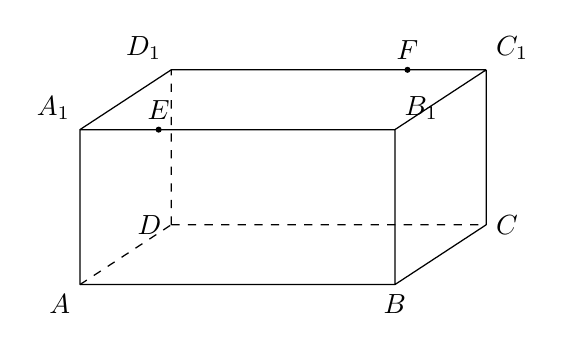
\begin{tikzpicture}[x={(1cm,0cm)},y={(0.58cm,0.38cm)},z={(0cm,0.82cm)},line width=0.45pt]
  \coordinate (A) at (0,0,0);
  \coordinate (B) at (4,0,0);
  \coordinate (C) at (4,2,0);
  \coordinate (D) at (0,2,0);
  \coordinate (Aone) at (0,0,2.4);
  \coordinate (Bone) at (4,0,2.4);
  \coordinate (Cone) at (4,2,2.4);
  \coordinate (Done) at (0,2,2.4);
  \coordinate (E) at (1,0,2.4);
  \coordinate (F) at (3,2,2.4);
  \draw (A)--(B)--(C) (A)--(Aone)--(Bone)--(B) (Bone)--(Cone) (Cone)--(C)
    (Aone)--(Done)--(Cone) (Done)--(F) (Aone)--(E);
  \draw[dashed] (A)--(D) (D)--(C) (D)--(Done);
  \foreach \p/\pos/\lab in {A/below left/A,B/below/B,C/right/C,D/left/D,Aone/above left/{A_1},Bone/above right/{B_1},Cone/above right/{C_1},Done/above left/{D_1},E/above/{E},F/above/{F}} {
    \node[\pos] at (\p) {$\lab$};
  }
  \fill (E) circle (1.1pt);
  \fill (F) circle (1.1pt);
\end{tikzpicture}
\end{center}
\nopagebreak[4]
\end{question}
\begin{question}
\gkti{20}已知椭圆 $C:\dfrac{x^2}{a^2}+\dfrac{y^2}{b^2}=1$（$a>b>0$）的离心率为 $\dfrac{\sqrt2}2$，点 $(2,\sqrt2)$ 在 $C$ 上。

(1) 求 $C$ 的方程；  
(2) 直线 $l$ 不经过原点 $O$，且不平行于坐标轴，$l$ 与 $C$ 有两个交点 $A,B$，线段 $AB$ 中点为 $M$，证明：直线 $OM$ 的斜率与直线 $l$ 的斜率乘积为定值。

\end{question}
\begin{question}
\gkti{21}已知 $f(x)=\ln x+a(1-x)$。

(1) 讨论 $f(x)$ 的单调性；  
(2) 当 $f(x)$ 有最大值，且最大值大于 $2a-2$ 时，求 $a$ 的取值范围。

\Needspace{0.4\textheight}
\end{question}
\begin{question}
\gkti{22}如图，$O$ 为等腰三角形 $ABC$ 内一点，$\odot O$ 与 $\triangle ABC$ 的底边 $BC$ 交于 $M,N$ 两点，与底边上的高 $AD$ 交于点 $G$，且与 $AB,AC$ 分别相切于 $E,F$ 两点。

(1) 证明：$EF\parallel BC$；  
(2) 若 $AG$ 等于 $\odot O$ 的半径，且 $AE=MN=2\sqrt3$，求四边形 $EBCF$ 的面积。
\nopagebreak[4]
\begin{center}% FIG:q22-triangle-circle
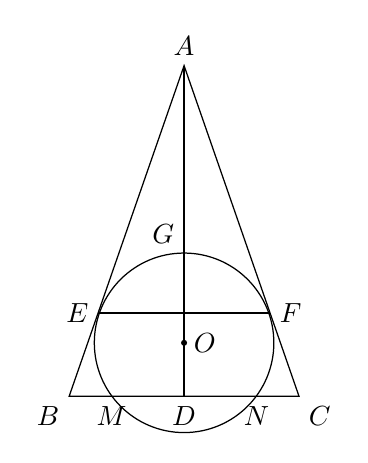
\begin{tikzpicture}[x=1cm,y=1cm,line width=0.45pt]
  \coordinate (A) at (0,4.2);
  \coordinate (B) at (-1.46,0);
  \coordinate (C) at (1.46,0);
  \coordinate (D) at (0,0);
  \coordinate (O) at (0,0.68);
  \coordinate (E) at (-1.09,1.06);
  \coordinate (F) at (1.09,1.06);
  \coordinate (G) at (0,1.82);
  \coordinate (M) at (-0.92,0);
  \coordinate (N) at (0.92,0);
  \draw (A)--(B)--(C)--cycle;
  \draw (0,4.2)--(0,0);
  \draw (O) circle[radius=1.14];
  \draw (E)--(F);
  \fill (O) circle (1.1pt);
  \foreach \p/\pos/\lab in {A/above/A,B/below left/B,C/below right/C,D/below/D,O/right/O,E/left/E,F/right/F,G/above left/G,M/below/M,N/below/N} {
    \node[\pos] at (\p) {$\lab$};
  }
\end{tikzpicture}
\end{center}
\nopagebreak[4]
\end{question}
\begin{question}
\gkti{23}在直角坐标系 $xOy$ 中，曲线 $C_1:\begin{cases}x=t\cos\alpha,\\y=t\sin\alpha,\end{cases}$（$t$ 为参数，$t\ne0$），其中 $0\le\alpha<\pi$。在以 $O$ 为极点，$x$ 轴正半轴为极轴的极坐标系中，曲线 $C_2:\rho=2\sin\theta$，$C_3:\rho=2\sqrt3\cos\theta$。

(1) 求 $C_2$ 与 $C_3$ 交点的直角坐标；  
(2) 若 $C_1$ 与 $C_2$ 相交于点 $A$，$C_1$ 与 $C_3$ 相交于点 $B$，求 $|AB|$ 的最大值。

\end{question}
\begin{question}
\gkti{24}设 $a,b,c,d$ 均为正数，且 $a+b=c+d$，证明：

(1) 若 $ab>cd$，则 $\sqrt a+\sqrt b>\sqrt c+\sqrt d$；  
(2) $\sqrt a+\sqrt b>\sqrt c+\sqrt d$ 是 $|a-b|<|c-d|$ 的充要条件。

\end{question}